\documentclass{beamer}
\mode<presentation>{\usetheme{AV}}
\usepackage{etex}
\usepackage[export]{adjustbox}
\usepackage{epsfig}
\usepackage{feynmp}
\usepackage{verbatim}
\usepackage{listings}
\usepackage{colortbl}

\usepackage{color}

\definecolor{mygreen}{rgb}{0,0.6,0}
\definecolor{mygray}{rgb}{0.5,0.5,0.5}
\definecolor{mymauve}{rgb}{0.58,0,0.82}

\lstset{ %
  backgroundcolor=\color{white},   % choose the background color; you must add \usepackage{color} or \usepackage{xcolor}
%  basicstyle=\footnotesize,        % the size of the fonts that are used for the code
  breakatwhitespace=false,         % sets if automatic breaks should only happen at whitespace
  breaklines=true,                 % sets automatic line breaking
  captionpos=b,                    % sets the caption-position to bottom
  commentstyle=\color{mygreen},    % comment style
  deletekeywords={...},            % if you want to delete keywords from the given language
  escapeinside={\%*}{*)},          % if you want to add LaTeX within your code
  extendedchars=true,              % lets you use non-ASCII characters; for 8-bits encodings only, does not work with UTF-8
  frame=single,                    % adds a frame around the code
  keepspaces=true,                 % keeps spaces in text, useful for keeping indentation of code (possibly needs columns=flexible)
  keywordstyle=\color{blue},       % keyword style
  language=Octave,                 % the language of the code
  morekeywords={*,...},            % if you want to add more keywords to the set
  numbers=left,                    % where to put the line-numbers; possible values are (none, left, right)
  numbersep=5pt,                   % how far the line-numbers are from the code
  numberstyle=\tiny\color{mygray}, % the style that is used for the line-numbers
  rulecolor=\color{black},         % if not set, the frame-color may be changed on line-breaks within not-black text (e.g. comments (green here))
  showspaces=false,                % show spaces everywhere adding particular underscores; it overrides 'showstringspaces'
  showstringspaces=false,          % underline spaces within strings only
  showtabs=false,                  % show tabs within strings adding particular underscores
  stepnumber=2,                    % the step between two line-numbers. If it's 1, each line will be numbered
  stringstyle=\color{mymauve},     % string literal style
  tabsize=2,                       % sets default tabsize to 2 spaces
  title=\lstname,                   % show the filename of files included with \lstinputlisting; also try caption instead of title
belowskip=-1.2em
}

\usepackage[utf8]{inputenc}
\usepackage[T1]{fontenc}
\usepackage{lmodern}
\usepackage{amsfonts}
\usepackage{supertabular}

\usepackage{textcomp}
\usepackage{amsmath}
\usepackage{amssymb}
\usepackage{graphicx}
%\usepackage{wrapfig}
\usepackage{subfigure}
\usepackage{type1cm}
\usepackage{tikz}
\usepackage{tikz-3dplot}
\usepackage{tikz}
\usepackage{tikz-3dplot}
\usepackage{pgfplots}
\usepackage{ulem}
\usetikzlibrary{shapes,arrows}
\usepackage{pgfplots}
\usetikzlibrary{shapes,arrows}
\usepackage{rotating}%     - to rotate boxes, pictures etc.
\usepackage{amsmath}%      - to use the AMS extended math package
\usepackage{amssymb}%      - to obtain additional math symbols in AMS fonts
\usepackage{amscd}%        - to obtain AMS flow chart utilities
\usepackage{array}%        - to obtain additional tabular functionality
\usepackage{multirow}%     - for multirow-entries in tables
\usepackage{supertabular}% - for multi-page tables
\usepackage{dcolumn}%      - decimal-point aligned colums in tables
\usepackage{xspace}%       - to add empty space after commands
\usepackage{upgreek}%      - provide upright greek letters
\usepackage{calc}%         - enhanced calculus in LaTeX macros
\usepackage{ifthen}%       - enhance logical structures in LaTeX macros
\usepackage{cite}%         - for multiple citations like [1-4] instead of [1,2,3,4]
\usepackage{tikz} 
%\usepackage{enumitem} 
\usepackage{multirow}
\usepackage{amssymb}
\usepackage{mathtools}
\usepackage{graphicx}


\def\Tiny{\fontsize{4.0pt}{4.0pt}\selectfont}

\title[DPHEP2017]{2nd Data Preservation in High Energy Physics Collaboration Meeting}
\subtitle[DPHEP2017]{DPHEP2017}
\author[Andrii Verbytskyi]{
Andrii Verbytskyi
}
\date[]{\\ \today}


\setbeamersize{text margin left=.3cm,text margin right=.3cm} 
\listfiles
\begin{document}

\usebackgroundtemplate{%
  \tikz\node [anchor=north east, inner sep=0pt,opacity=0.18]  at (current page.center)
     {\includegraphics[height=0.5\paperheight,width=\paperwidth]{bkg3.eps}};
}

\frame{
\vspace{0.3cm}
\begin{figure}

\includegraphics[height=1.0cm]{eps/MPP_os_logo_cmyk.eps}
%\includegraphics[height=1.0cm]{eps/CERN-Logo-cyan-RGB_ger.eps}
\hspace*{12.0cm}
\end{figure}
\begin{center}
\vspace{1.3cm}
{\LARGE The OPAL long term data preservation projects in Max-Planck Institute f\"{u}r Physik}
\vspace{0.3cm}
\end{center}
\begin{center}
\vspace{0.3cm}
Andrii Verbytskyi\\
\end{center}
\vspace{1.0cm}
\begin{center}
\footnotesize  2nd Data Preservation in High Energy Physics Collaboration Meeting \\Geneve,\\ \today
\end{center}
\vspace{0.4cm}
}


\usebackgroundtemplate{%
  \tikz\node [anchor=north east, inner sep=0pt,opacity=0.98]  at (current page.center)
     {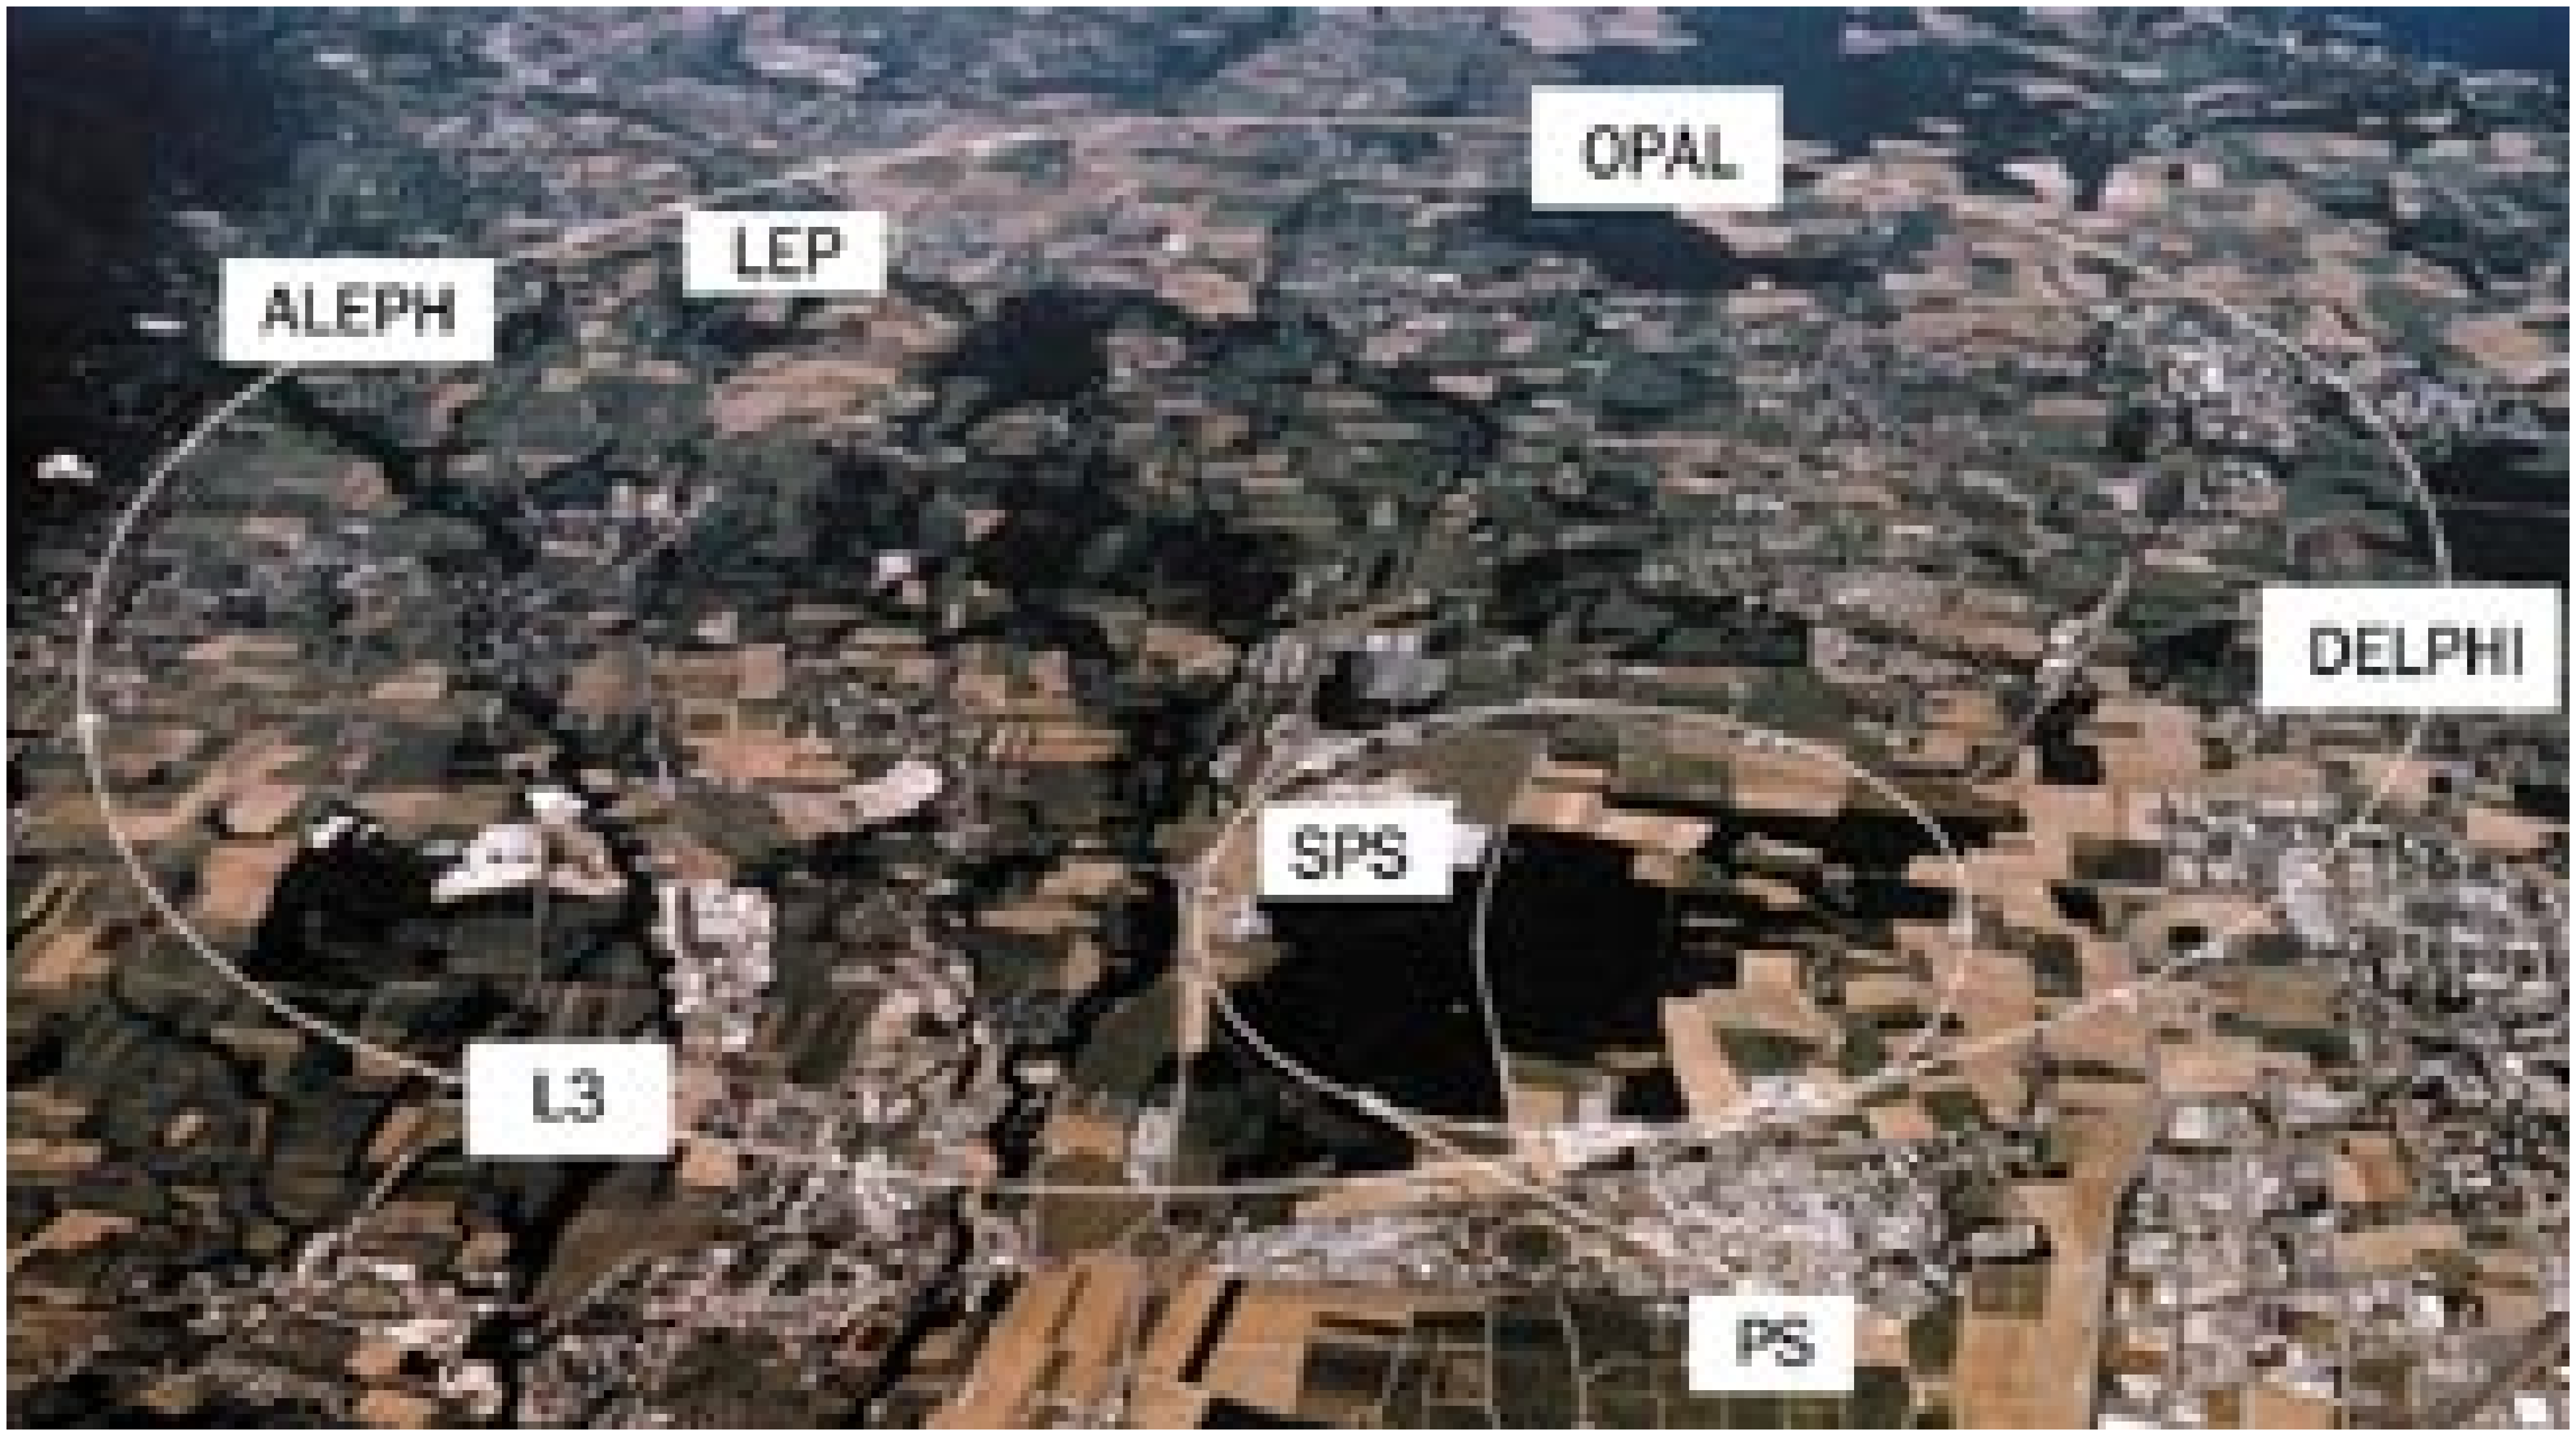
\includegraphics[height=1.0\paperheight,width=\paperwidth]{LEP}};
}


\frame{\frametitle{LEP}
{\color{white}\Large\bf 
\begin{itemize} 
\item \color{white} Electron-positron collider, started in 1979 in CERN; 
\item \color{white}2.3km ring, beam energies up to 23GeV;
\item \color{white}Experiments: ALEPH, DELPHI, L3, {\color{red}OPAL}.
\end{itemize} 
} 
}
\usebackgroundtemplate{}

\frame{\frametitle{OPAL}
\begin{centering}
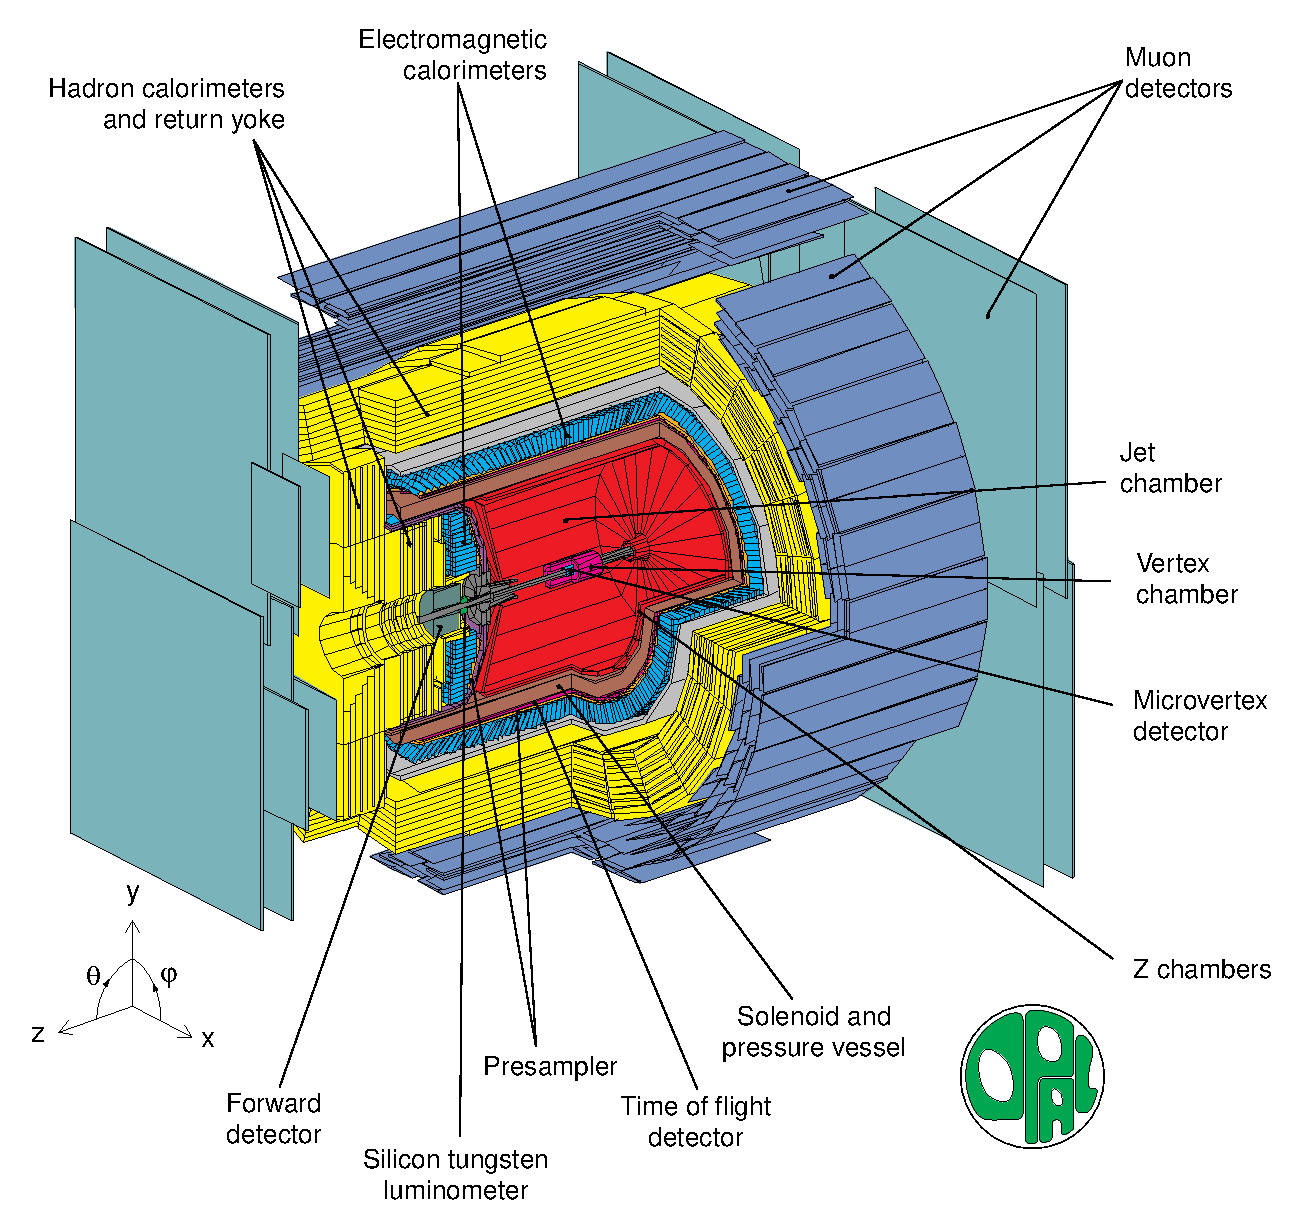
\includegraphics[width=0.8\linewidth]{opal_3d_colour}	
\end{centering}
%\begin{columns}[c]
%\column{0.49\linewidth}
%\begin{itemize} 
%\item multipurpose detector 
%\item large solid angle coverage
%\item digital readout
%\end{itemize} 
%\column{0.49\linewidth}
%\begin{itemize} 
%\item advanced tracking system
%\item calorimeter
%\item muon chambers
%\end{itemize} 
%\end{columns}
%{\bf \color{red} 35 years later: still unique energy range coverage!}
}


%eps/OPALDet.eps

\usebackgroundtemplate{%
  \tikz\node [anchor=north east, inner sep=0pt,opacity=0.18]  at (current page.center)
     {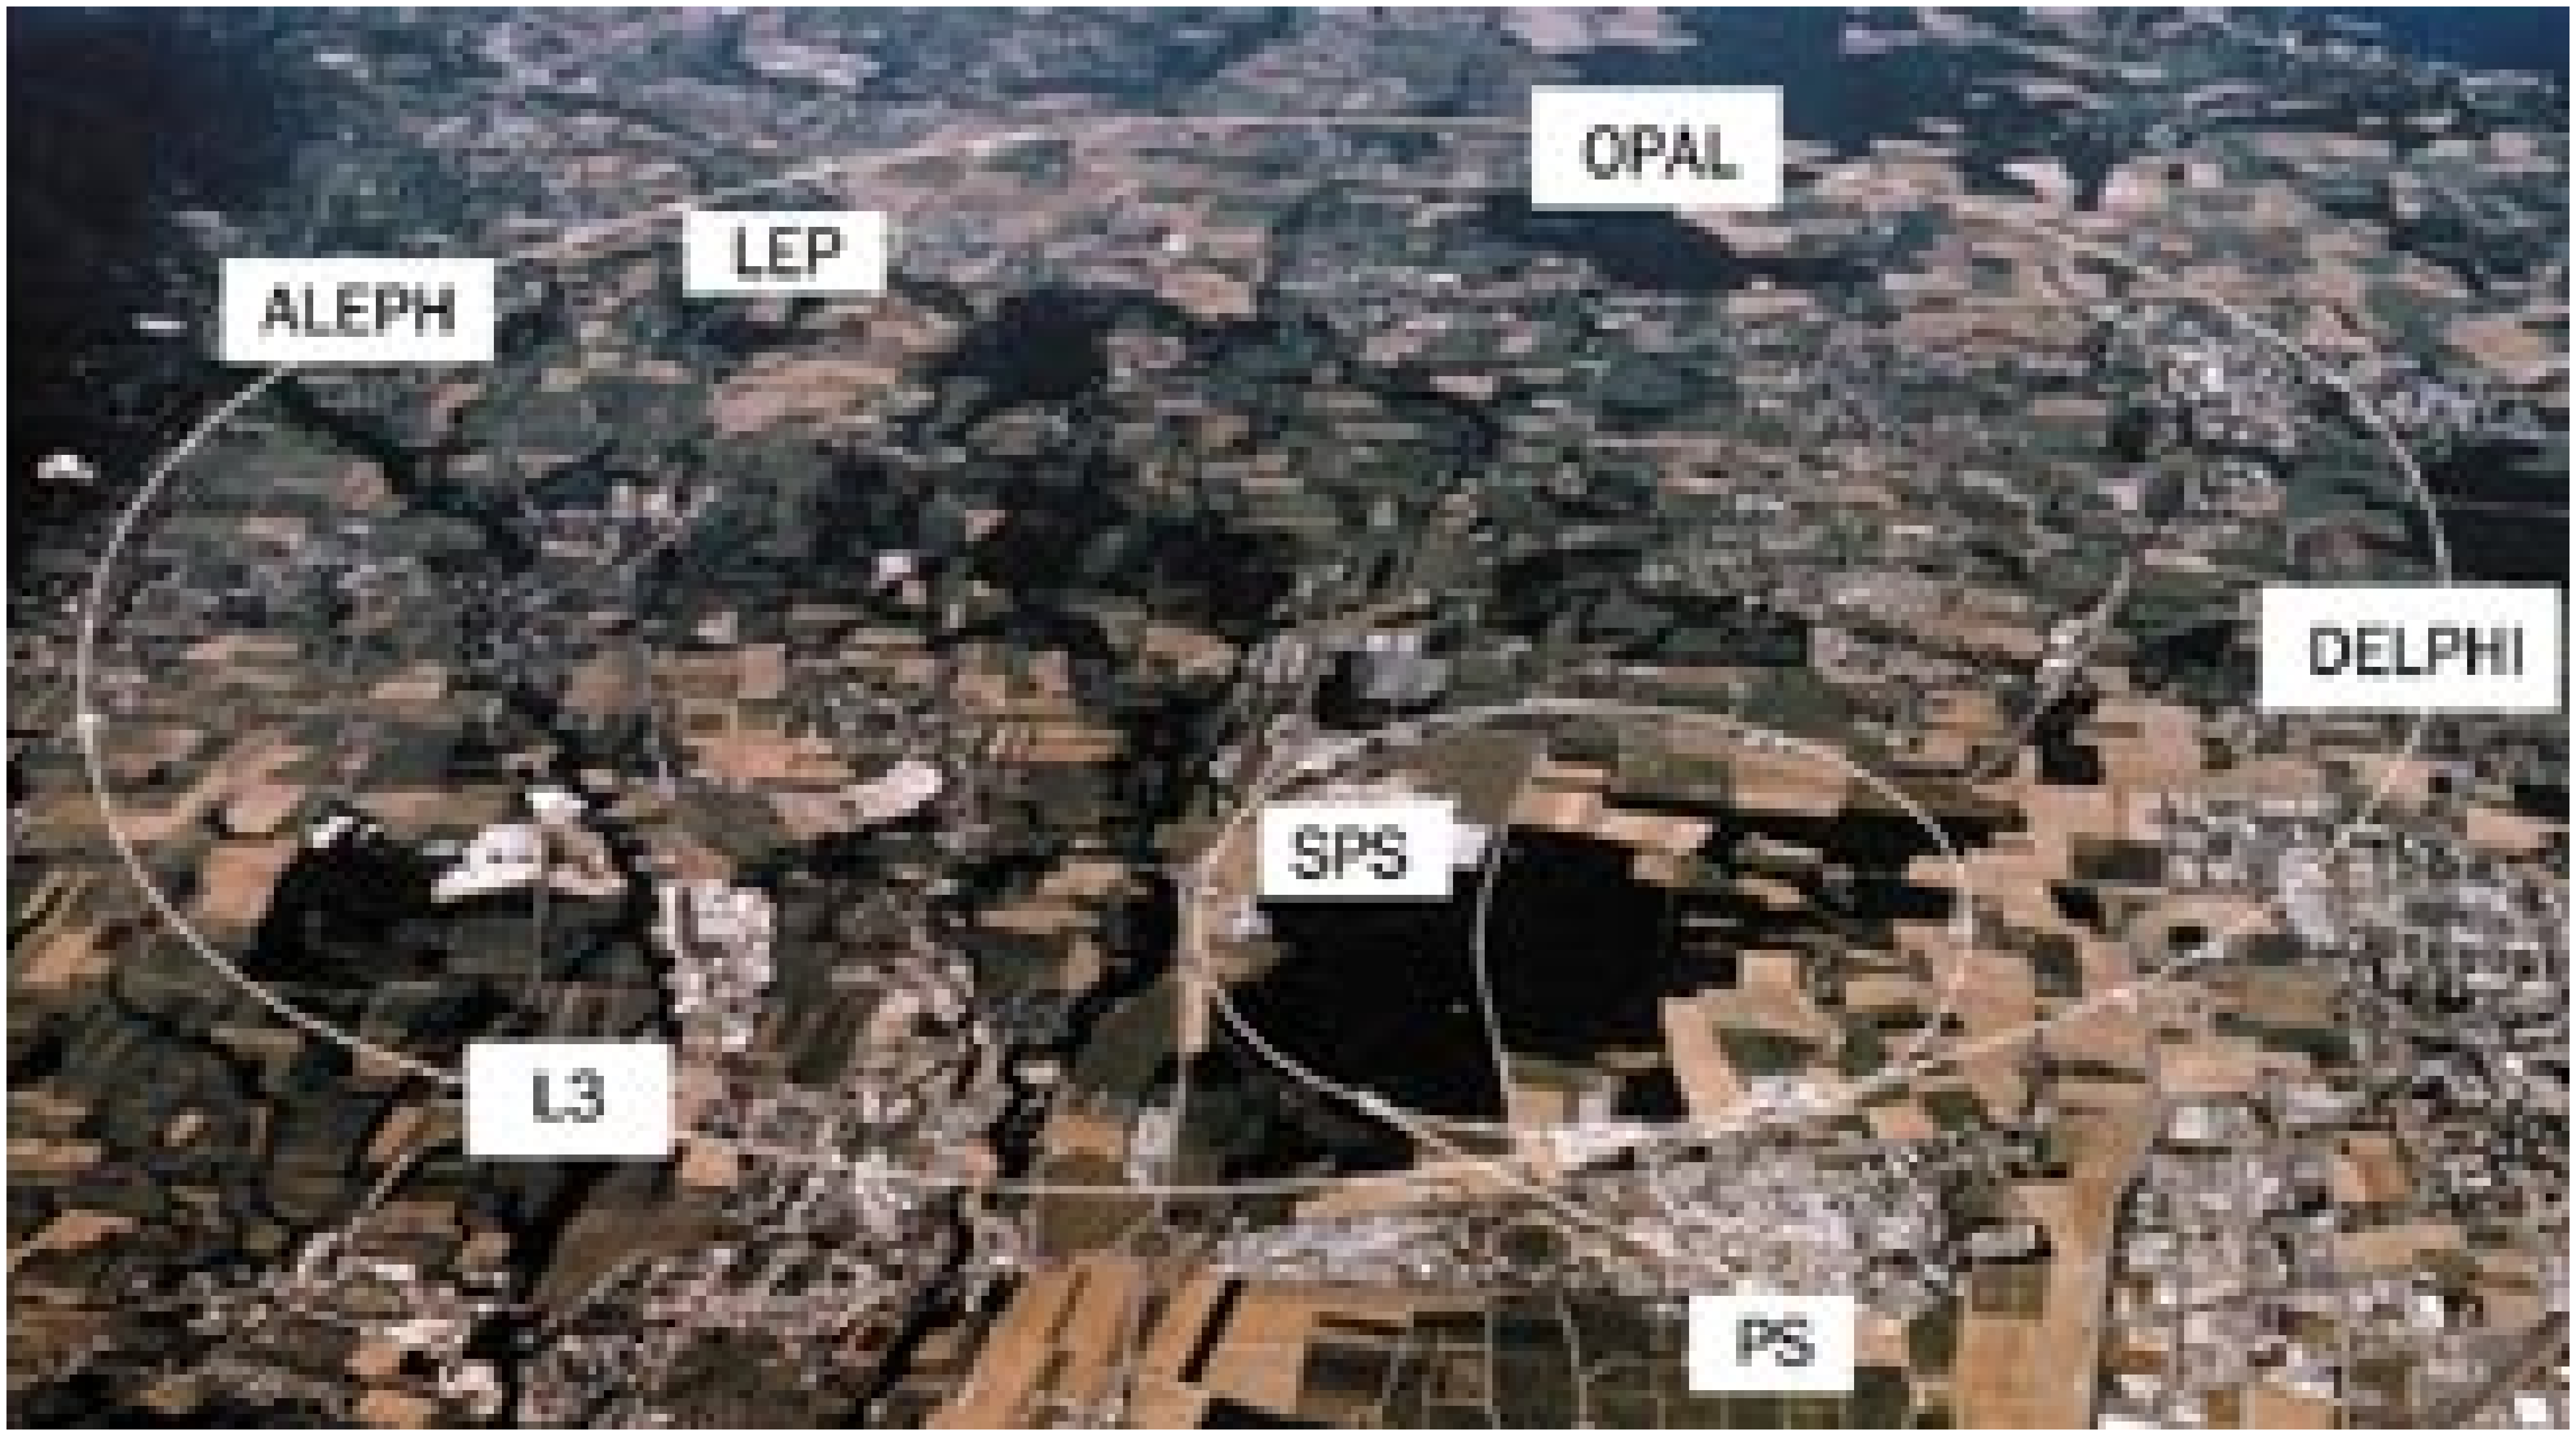
\includegraphics[height=1.0\paperheight,width=\paperwidth]{LEP}};
}


\frame{\frametitle{OPAL  and data preservation}
\begin{columns}[c]
\column{0.54\linewidth}
OPAL@LEP reminder:
\begin{itemize}
\item Precision QCD, electroweak physics.%: discovery of gluon, $\alpha_{s}$ measurements.
%{\bf 
%\item {\bf  The oldest and  most successful  Data Preservation effort!}
\end{itemize}
Motivation for data preservation:
\begin{itemize}
\item Future data (re-)analysis with new models and new approaches.
\item Modelling for the future experiments.
%\item Outreach and education.
%\item {\bf Exceptional example of preservation of 30y.o. data.}
\end{itemize}
\column{0.45\linewidth}
%\includegraphics[width=1.0\linewidth]{eps/OPAL-ID-records.eps}
\end{columns}
}

\usebackgroundtemplate{}








\frame{\frametitle{MPP DP  model for OPAL}
\begin{columns}[c]
	\column{0.6\linewidth}
%{\centering \bf \color{red}\Large Yes, 11 papers!}\\
{\bf Data preservation is about  new and interested results with old data.}
%A lot of amazing results was obtainded with preserved data in 1995-2013.\\
{\bf In adiition  the Data Preservation  experince with OPAL has an extreame importance on itself.}\\
In out model we describe  ingredients and tools:\\
\column{0.4\linewidth}
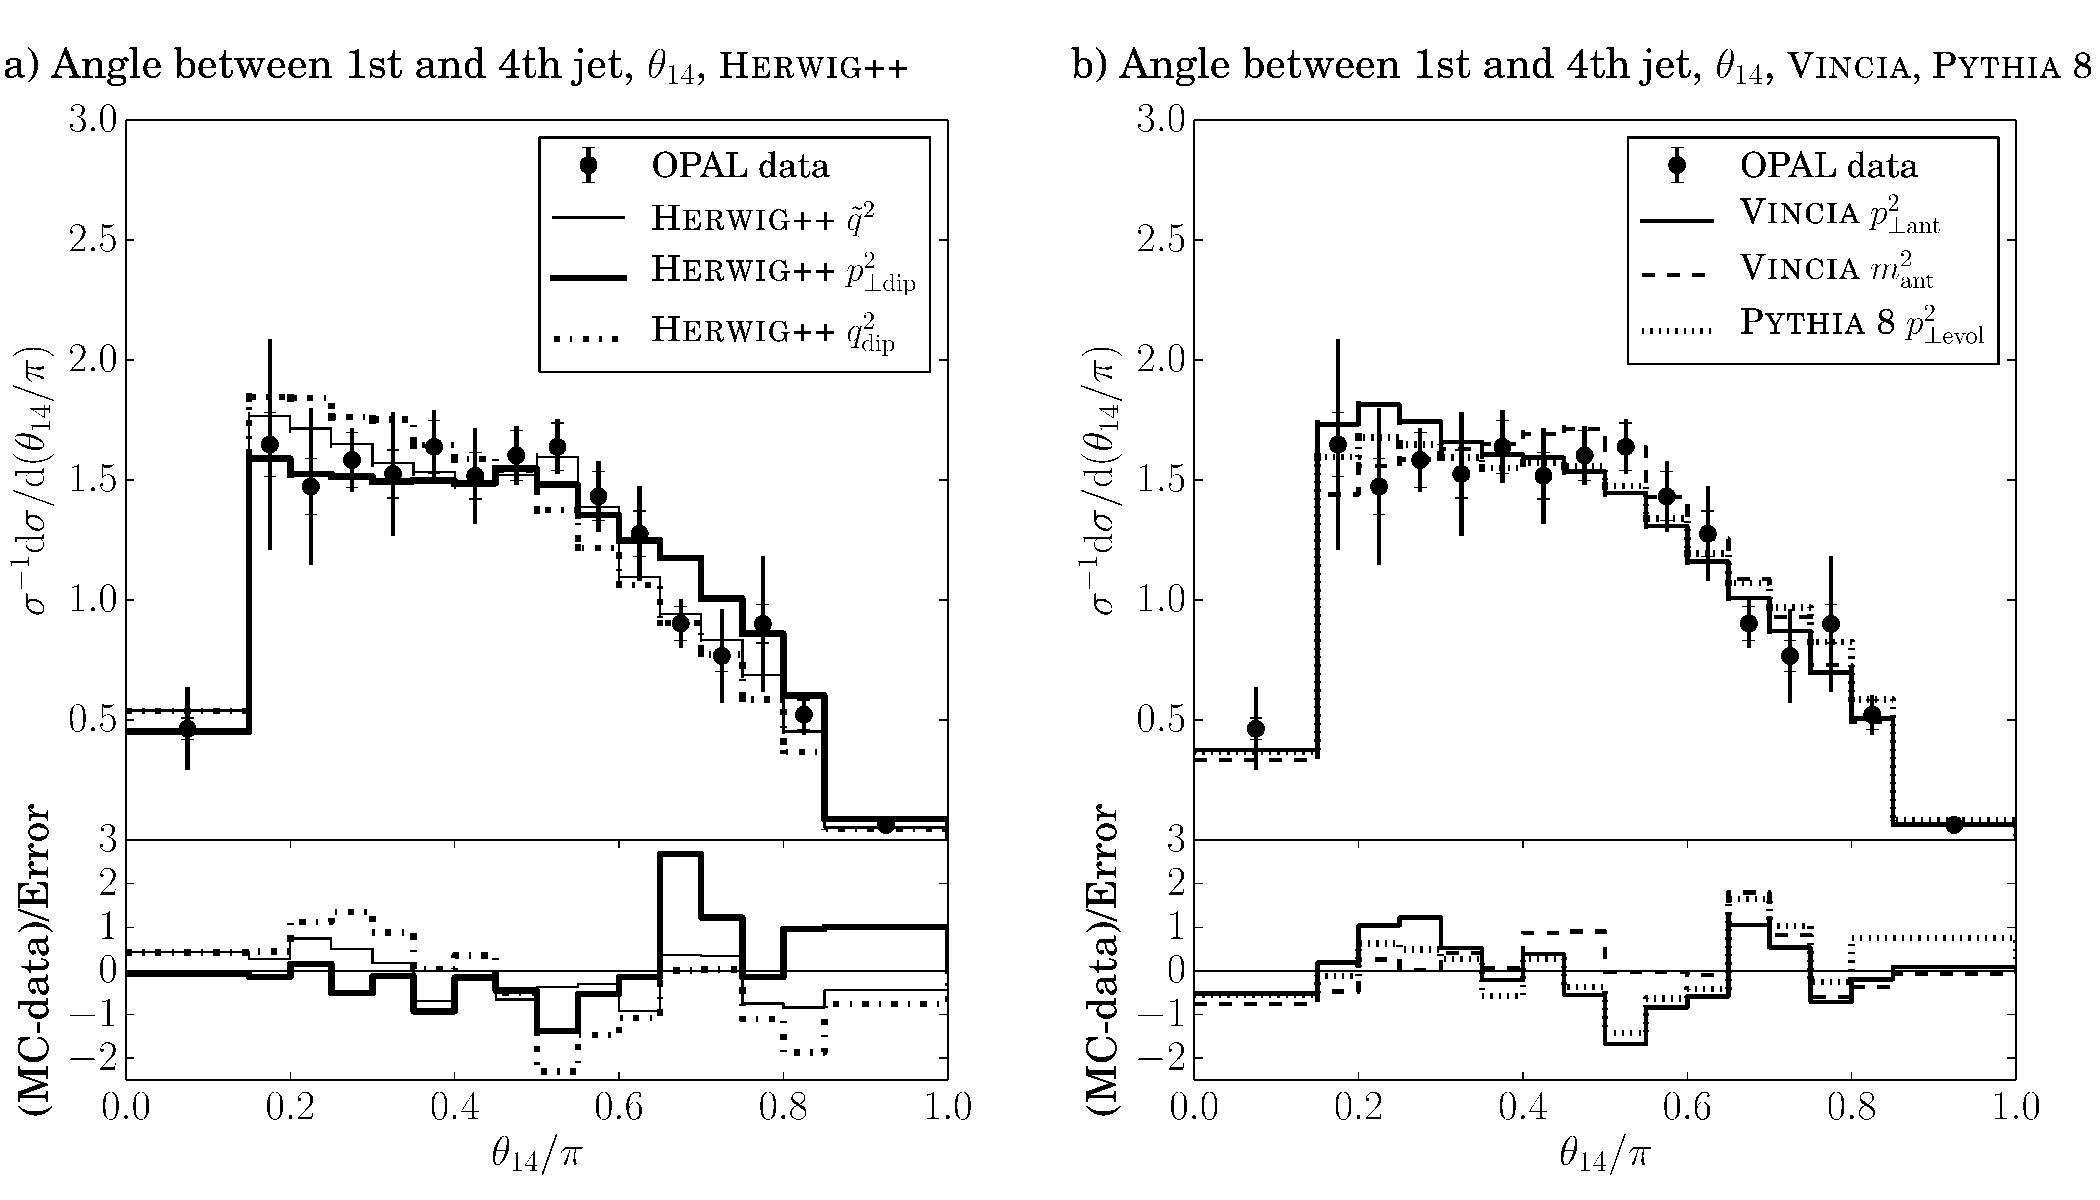
\includegraphics[width=1.0\linewidth,height=0.85\linewidth]{A14.ps}\\
Eur.Phys.J. C75 (2015) no.12, 571
\end{columns}
\begin{columns}[c]
\column{0.4\linewidth}
\begin{itemize}
\item Data bits
\item Software
\end{itemize}
\column{0.6\linewidth}
\begin{itemize}
\item Experiment documentation
\item DP policies and  documentation
\end{itemize}
\end{columns}

\begin{itemize}
\item But in the end we are interested in {\bf physics }.
\end{itemize}

Main idea: enable physics and make it doable with modern methods in modern environments with minimal effort.\\
}



\frame{\frametitle{MPP DP model for documentation  and policies}
%MPP data preservation relies on the documentation preserved as papers by CERN/CERN library/InSpire.\\
\begin{itemize}
\item OPAL publications are available in InSpire, journals, arXiv or in CERN.
\item The non-digital documentation is preserved in CERN.
%\item Logbooks included!
%\item Some available online as well, see details at https://wwwOPAL.mpp.mpg.de/
\end{itemize}
\begin{figure}\centering
%\includegraphics[width=0.3\linewidth]{eps/OPAL_Logbook.eps}
\end{figure}
}

\frame{\frametitle{MPP DP model for OPAL data bits }
\begin{itemize}
\item OPAL data are stored in CERN and in MPCDF on locally accessible tapes and in disk pool.
\item Access via multiple protocols with grid tools worldwide to disk pools.
%\item Grid-enabled storage for new samples (Monte Carlo) and analysis is available.
\item Straightforward procedure to add new (MC) samples.
%\item In the end nowadays all the data from OPAL can fit to a modern USB stick.
\end{itemize}
%\begin{figure}\centering
%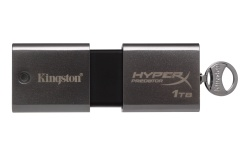
\includegraphics[width=0.25\linewidth]{eps/USB.eps}
%\end{figure}
}


%\footnote{Because of data reshiffling now H1 data temporary is only on tape}	


\frame{\frametitle{OPAL data in MPP: Bits statistics}
%\hspace{6cm}
\begin{columns}[c]
\column{0.85\linewidth}
Data are  ROOT/PAW ntuples, ASCII files, etc. Particle level NLO Monte Carlo is available for multiple generators.
\begin{table}\centering\bf\begin{tabular}{|c|c|c|}\hline
{\color{maroon}           } & {\color{maroon}   MPCDF     }          \\\hline\hline
{\color{maroon}Files:      }&{\color{maroon}   5.4k  } \\
{\color{maroon}Volume:     }&{\color{maroon}   $600 GB$ ($645\times10^{9}$ bytes)} \\
{\color{maroon}Work area:  }&{\color{maroon}    yes       } \\
{\color{maroon}Access:     }&{\color{maroon}   Worldwide  } \\
{\color{maroon}Protocols: } &{\color{maroon}   Multiple, see list   } \\
{\color{maroon}Auth:      } &{\color{maroon}   Grid certificate with OPAL VO membership } \\\hline
\end{tabular}
\end{table}
\column{0.15\linewidth}
\rotatebox{90}{
\includegraphics[height=0.40\linewidth,width=2.8\linewidth]{eps/MPCDF}}
\end{columns}


Available at:
\begin{itemize}
\item gsidcap://grid-srm.rzg.mpg.de:22128/pnfs/rzg.mpg.de/data/opal
\item grid-gftp2.rzg.mpg.de 
\item davs://grid-dav.rzg.mpg.de:2880//opal
\item \dots
\end{itemize}

}





\frame{\frametitle{MPP model for software preservation}
Explicit effort put to make software it work in the next 10-15 years.
Previous efforts and high quality of code made it possible.%  porting  was possible.

Key ideas:
\begin{itemize}
\item Rely on industry, not HEP-only standards.
\item Enable integration and compatibility with new physics software, e.g. data bases and Monte Carlo generators.
%\item ISO image of full operating system relying on Intel $x86$  architecture to assure easy usage.
\item {\bf i.e.\ make software analysis-ready}
\end{itemize}


}






\frame{\frametitle{OPAL software in MPP}
\begin{itemize}
\item Full chain for reconstruction of raw data to PAW/ROOT ntuples was resurrected.
\item Main software for the analysis of early preserved and reconstructed data is vanilla PAW or ROOT(via h2root).
\item Additional software includes:
\begin{itemize}
\item event display;
\item Monte-Carlo generation packages;
\end{itemize}
\end{itemize}
}



\frame{\frametitle{OPAL software porting quest in detail}
Not much to say\dots But that is good!
\begin{columns}[c]
\column{0.5\linewidth}
\begin{itemize}
\item High quality code.
\end{itemize}
\column{0.5\linewidth}
\begin{itemize}
\item Huge and {\bf \color{red} successful } effort by Matthias Schr\"{o}der to keep the code compatible with modern systems.
\end{itemize}
\end{columns}
\begin{itemize}
\item Tests to put software in VM were done. Things are working, but no image so far. Biggest problem is event display.
\end{itemize}
}



\frame{\frametitle{OPAL software extension}
One can go ZEUS/JADE way:
\begin{itemize}
\item 	Add modern MC generators and converstion utility for modern format. Easy: OPAL uses ASCII bases format.
\item   Add virtualization.
\end{itemize}
Not completed, but one can imagine how things should look like.
}

\section{Conclusions}

\frame{\frametitle{MPP Data Preservation summary}
\begin{itemize}
\item Huge work was done to preserve OPAL data and software.
\item Data is accessible in  MPCDF and software is {\bf\color{red}analysis-ready}.
\item Virtualization is on the way.
\item {So far MPP is involved mainly in the analysis
\begin{itemize}
\item Jet physics.
\item Collective phenomena.
\end{itemize}
}
\end{itemize}

}
\section{Data Preservation applications}
\frame{\frametitle{OPAL Data Preservation applications}
\begin{itemize}
\item Hodronisation/non-perturbative effects.
\item Fundamantal quaestions of QCD.
\item Exotic hadronic states.
\item Flavour physics.
\item \dots
\end{itemize}
}

\section{What other experiments can learn from OPAL DP}


\frame{\frametitle{Software}
\begin{itemize}
\item Quality of code is important.
\item Compatibility with modern experiments!
\item Involvement of experts (M.Schroeder)
\item Promotion: an anecdotal case of spending two conference evenings advertising preserved LEP data and its avialibility for re-analysis.
\end{itemize}
}



\frame{\frametitle{This part should be considered as an opinion}



}



\frame{\frametitle{Some thoughts on DP in general}
%OK, OPAL DP is quite advanced. But, in the same time, the collaboration has ended in 2007.
%10 years is enough to understand the chalanges of analysis of data after 10 years..
Some technical problems:
\begin{itemize}
\item Missing or obscure  technical documantation. While OPAL primer does exist, it doesn't cover everything.
Thought one can admitt the documantation from OPAL is quite good.
\item Quite oftern even the physics of old experimants is forgotten.
e.g.\ absence of jet $p_{T}$ cut in $e^{+}e^{-}$ confuses people working with hadronic colliders.


\item The terminology in 2000 and now is different, old methods are renamed, etc.    This slows down communication.
e.g.\ Monte Carlo tuning method by DELPHI (Z. Phys., C73 (1996) 11-60) has 293 citations overall, 2 in 2016.
The tool based on the method
   Professor (Eur.Phys.J. C65 (2010) 331-357) has 217 citations overall 22 in 2016.
Ironically datasets from DELPHI are intensively used with the framework.
\end{itemize}
}

\frame{\frametitle{Some thoughts on OPAL and more}
More sociological problems:
\begin{itemize}
\item Manpower in not actually that severe problem per se. But the concentration is.
 With low spatial concentration of knowledge, there are few people that can be asked about specific things, discussions via mail excahnge are not that productive.
The learning curve becomes too long. Should bigger laboratories like CERN and DESY be more involved? Some events for young physicists?        
\item Long duration of any potential analysis because of envolvement of members in other progects. The duratin of any analysis more than 12 months 
implies that it cannot be advertised as a master or bachelor thesis. This rejects a very important source of manpower or requires more intensive supervision that for the 
running experiemnts. Could multiple supervisors and multiple master studens  per  project be a solution? Thought the publication of the result should be mandaratory.

%\item In the end DP has some sociological problems as well.
\end{itemize}

}

\frame{\frametitle{Some thoughts on OPAL and more}
\begin{itemize}
\item Often the investments of manpower in earliest and not very precise measurements are much bigger than investments in the DP or even in the later results.
Emphasise of DP importance could fix this imbalance and make later/after OEDT precise analyses easier.
\item A bit of sociological problem.

%\item In the end DP has some sociological problems as well.
\end{itemize}

}


\end{document}

